% The VMDance quick-start guide (Supporting Information of the JCIM article).
% Build: make (latexmk, pdflatex). Its numbers are in numbers.tex, made by
% numbers.tcl from the guide's own script, quickstart.tcl (make numbers).
% Its figures are in figures/, made by figures.tcl from the same script (make
% figures); the workflow and the algorithms' diagrams and the logo are the
% online documentation's (../docs/_static), read only.
\documentclass[11pt,letterpaper]{article}

\usepackage[T1]{fontenc}
\usepackage[utf8]{inputenc}
\usepackage{libertinus}
\usepackage[scaled=0.92,varqu,varl]{inconsolata}
\usepackage{amssymb}
\usepackage[margin=1in,headheight=14pt]{geometry}
\usepackage{microtype}
\usepackage{graphicx}
\usepackage{xcolor}
\usepackage{booktabs,tabularx,array}
\usepackage{enumitem}
\usepackage{listings}
\usepackage[most]{tcolorbox}
\usepackage{titlesec}
\usepackage{fancyhdr}
\usepackage[font=small,labelfont={bf,sf},labelsep=period]{caption}
\usepackage{subcaption}
\usepackage{float}
\usepackage{multicol}
\usepackage{tikz}
\usepackage[hyphens]{url}
\usepackage[colorlinks,linkcolor=accent,urlcolor=accent,citecolor=accent,
            pdftitle={VMDance quick-start guide},
            pdfsubject={Clustering molecular dynamics trajectories in VMD with MDANCE's algorithms}]{hyperref}

% file names, breakable after _ . /
\def\UrlBreaks{\do\_\do.\do/}
\newcommand{\file}[1]{\path{#1}}
\graphicspath{{figures/}{../docs/_static/diagrams/}{../docs/_static/logo/}}
% The quick-start guide's numbers, made by numbers.tcl (make numbers):
% its script, quickstart.tcl, run on the tau peptide of BitQT's examples. Do not edit.
\newcommand{\qsVMD}{2.0.0a6}
\newcommand{\qsArch}{MACOSXARM64}
\newcommand{\qsTcl}{8.6.18}
\newcommand{\qsBackendCommit}{a5d197b}
\newcommand{\qsMinutes}{1}
\newcommand{\qsMachine}{Apple M1 Max}
\newcommand{\qsVersion}{1.0a1}
\newcommand{\qsFrames}{6001}
\newcommand{\qsAtoms}{50}
\newcommand{\qsFitFrame}{1000}
\newcommand{\qsFitWorst}{1e-05}
\newcommand{\qsFitMean}{3.69}
\newcommand{\qsAsIs}{3.33}
\newcommand{\qsFitted}{3.30}
\newcommand{\qsSuperposed}{1}
\newcommand{\qsElbowRows}{2 & 2464 & 1.52 & 29\% & 1.00 \\
3 & 1757 & 1.87 & 37\% & 0.77 \\
4 & 1465 & 1.91 & 42\% & 0.76 \\
5 & 1261 & 1.79 & 46\% & 0.60 \\
6 & 1146 & 1.90 & 49\% & 0.78 \\
7 & 1033 & 2.13 & 51\% & 0.63 \\
8 & 947 & 2.05 & 53\% & 0.70 \\
9 & 893 & 1.99 & 54\% & 0.74 \\
10 & 844 & 1.91 & 56\% & 0.61 \\
11 & 787 & 1.95 & 57\% & 0.66 \\
12 & 764 & 1.90 & 58\% & 0.68}
\newcommand{\qsDbLowest}{2}
\newcommand{\qsDbLowestValue}{1.52}
\newcommand{\qsChHighest}{2}
\newcommand{\qsChHighestValue}{2464}
\newcommand{\qsChFirst}{2464}
\newcommand{\qsChLast}{764}
\newcommand{\qsKFirst}{2}
\newcommand{\qsKLast}{12}
\newcommand{\qsDbDip}{5}
\newcommand{\qsDbDipValue}{1.79}
\newcommand{\qsDbDipBeforeK}{4}
\newcommand{\qsDbDipBefore}{1.91}
\newcommand{\qsDbDipAfterK}{6}
\newcommand{\qsDbDipAfter}{1.90}
\newcommand{\qsDbDipStability}{0.60}
\newcommand{\qsStable}{2}
\newcommand{\qsStableValues}{1.00}
\newcommand{\qsAboveFrom}{3}
\newcommand{\qsAboveMin}{0.60}
\newcommand{\qsAboveMax}{0.78}
\newcommand{\qsSuggestWords}{Davies--Bouldin: lowest at k 2, sharpest dip at k 5; Calinski--Harabasz: highest at k 2; seedings agree (0.9 or more) at k 2}
\newcommand{\qsK}{6}
\newcommand{\qsKStability}{0.78}
\newcommand{\qsKCh}{1146}
\newcommand{\qsKDb}{1.90}
\newcommand{\qsStayMin}{1.5}
\newcommand{\qsStayMax}{1.8}
\newcommand{\qsRunOne}{KMeans NANI, k 6 $\rightarrow$ 6 clusters}
\newcommand{\qsSizes}{691, 1229, 913, 1376, 748 and 1044}
\newcommand{\qsPcts}{12, 20, 15, 23, 12 and 17}
\newcommand{\qsReps}{3618, 4632, 5469, 3097, 4528 and 5368}
\newcommand{\qsCH}{1146}
\newcommand{\qsDB}{1.90}
\newcommand{\qsSilCentroid}{0.26}
\newcommand{\qsSilPairs}{0.27}
\newcommand{\qsSilNegative}{512}
\newcommand{\qsSilNegativePct}{9}
\newcommand{\qsHalfFirst}{3000}
\newcommand{\qsHalfSecond}{3001}
\newcommand{\qsDivergence}{0.011}
\newcommand{\qsDiffCluster}{4}
\newcommand{\qsDiffPoints}{7}
\newcommand{\qsDiffFirst}{477}
\newcommand{\qsDiffSecond}{271}
\newcommand{\qsDiffFirstPct}{16}
\newcommand{\qsDiffSecondPct}{9}
\newcommand{\qsBothVisitAll}{1}
\newcommand{\qsCompareWords}{first and second: divergence 0.011 (0: the same shares of the clusters; 0.69: no cluster in common); cluster 4 differs most, 15.9\% of first against 9.0\% of second}
\newcommand{\qsMapOne}{40}
\newcommand{\qsMapTwo}{14}
\newcommand{\qsDivineLabel}{DIVINE, k 6 $\rightarrow$ 6 clusters}
\newcommand{\qsDivineClusters}{6}
\newcommand{\qsDivineSizes}{1155, 1109, 843, 1325, 662 and 907}
\newcommand{\qsDivineNoise}{0}
\newcommand{\qsDivineAri}{0.54}
\newcommand{\qsHelmLabel}{HELM, k 6 $\rightarrow$ 6 clusters}
\newcommand{\qsHelmClusters}{6}
\newcommand{\qsHelmSizes}{369, 745, 1135, 805, 1429 and 1518}
\newcommand{\qsHelmNoise}{0}
\newcommand{\qsHelmAri}{0.45}
\newcommand{\qsEqualLabel}{eQual, radius 8 $\rightarrow$ 8 clusters}
\newcommand{\qsEqualClusters}{8}
\newcommand{\qsEqualSizes}{4694, 784, 401, 62, 35, 19, 3 and 2}
\newcommand{\qsEqualNoise}{1}
\newcommand{\qsEqualAri}{0.09}
\newcommand{\qsSweepBest}{KMeans NANI, k 2, StratAll}
\newcommand{\qsSweepBestDb}{1.52}
\newcommand{\qsSweepConfigs}{42}
\newcommand{\qsSweepNotRun}{0}
\newcommand{\qsEqualTopThree}{4694, 784 and 401}
\newcommand{\qsEqualTopThreePct}{98}
\newcommand{\qsRuns}{4}
\newcommand{\qsExportFiles}{tau\_clusters.csv, tau\_distances.csv, tau\_labels.csv, tau\_residence.csv, tau\_silhouette.csv, tau\_summary.txt, tau\_timeline.csv, tau\_top\_frames.csv, tau\_transitions.csv, tau\_tree.csv}
\newcommand{\qsSessionKB}{775}

% The quick-start guide's benchmark, made by bench.tcl (make bench): the
% program against the library, medians of 3 runs. Do not edit.
\newcommand{\bnFrames}{6001}
\newcommand{\bnAtomsBackbone}{50}
\newcommand{\bnAtomsAll}{217}
\newcommand{\bnReps}{3}
\newcommand{\bnFitFrame}{999}
\newcommand{\bnMachine}{Apple M1 Max}
\newcommand{\bnRows}{KMeans NANI, k 6 & 50 & 1.11 & 1.43 & 0.8\(\times\) \\
DIVINE, k 6 & 50 & 1.07 & 1.44 & 0.7\(\times\) \\
HELM, k 6 (from 60) & 50 & 1.59 & 1.94 & 0.8\(\times\) \\
eQual, radius 8 & 50 & 1.09 & 1.50 & 0.7\(\times\) \\
Elbow scan, k 2 to 12 & 50 & 2.69 & 2.60 & 1.0\(\times\) \\
Elbow scan with stability & 50 & 24.3 & 22.2 & 1.1\(\times\) \\
KMeans NANI, k 6 & 217 & 4.16 & 5.25 & 0.8\(\times\) \\
DIVINE, k 6 & 217 & 3.97 & 5.38 & 0.7\(\times\) \\
HELM, k 6 (from 60) & 217 & 6.65 & 7.94 & 0.8\(\times\) \\
Elbow scan, k 2 to 12 & 217 & 12.1 & 11.7 & 1.0\(\times\)}
\newcommand{\bnCompared}{10}
\newcommand{\bnSame}{10}
\newcommand{\bnGainMin}{0.7}
\newcommand{\bnGainMax}{1.1}
\newcommand{\bnKmeansCli}{1.11}
\newcommand{\bnKmeansLib}{1.43}
\newcommand{\bnKmeansAllCli}{4.16}
\newcommand{\bnKmeansAllLib}{5.25}
\newcommand{\bnStabilityCli}{24.3}
\newcommand{\bnStabilityLib}{22.2}
\newcommand{\bnMemCli}{38}
\newcommand{\bnMemLib}{1206}


% Colours: the documentation's blue; VMD's title colours for the logo's letters
\definecolor{accent}{HTML}{1F5FAE}
\definecolor{muted}{HTML}{5A6270}
\definecolor{codebg}{HTML}{F4F6F9}
\definecolor{coderule}{HTML}{C5D0DE}
\definecolor{codecomment}{HTML}{5F7A55}
\definecolor{codestring}{HTML}{9A4A2E}
\definecolor{notebg}{HTML}{EEF3FA}
\definecolor{warnbg}{HTML}{FBF1E6}
\definecolor{warnrule}{HTML}{C98A3D}

% Headings and pages
\titleformat{\section}{\sffamily\Large\bfseries\color{accent}}{\thesection}{0.6em}{}
\titleformat{\subsection}{\sffamily\large\bfseries}{\thesubsection}{0.6em}{}
\titlespacing*{\section}{0pt}{2.2ex plus 0.6ex minus 0.3ex}{1.0ex}
\titlespacing*{\subsection}{0pt}{1.8ex plus 0.5ex minus 0.3ex}{0.6ex}
\pagestyle{fancy}
\fancyhf{}
\fancyhead[L]{\small\sffamily\color{muted}VMDance quick-start guide}
\fancyhead[R]{\small\sffamily\color{muted}\thepage}
\renewcommand{\headrulewidth}{0.3pt}
\setlist{itemsep=0.25ex,topsep=0.6ex}
\setlength{\parindent}{0pt}
\setlength{\parskip}{0.55ex plus 0.2ex}

% What the window shows, and a path through its menus: \ui{File}\then\ui{Save session}
\newcommand{\ui}[1]{\textsf{\textbf{#1}}}
\newcommand{\then}{\,\raisebox{0.15ex}{\scalebox{0.6}{$\blacktriangleright$}}\,}
\newcommand{\cmd}[1]{\texttt{#1}}
\newcommand{\Asq}{\AA\textsuperscript{2}}
\newcommand{\meta}[1]{\textrm{\emph{#1}}}

% Code
\lstdefinestyle{base}{
  basicstyle=\ttfamily\small, columns=fullflexible, keepspaces=true,
  backgroundcolor=\color{codebg}, frame=leftline, rulecolor=\color{coderule},
  framerule=2pt, xleftmargin=6pt, framexleftmargin=6pt, aboveskip=1.0ex,
  belowskip=0.6ex, showstringspaces=false, breaklines=true, upquote=true,
  commentstyle=\color{codecomment}, stringstyle=\color{codestring},
  keywordstyle=\bfseries}
\lstdefinestyle{tcl}{style=base, language=tcl,
  morekeywords={vmdance,mol,animate,atomselect},
  morecomment=[l]{;\#}}
\lstdefinestyle{sh}{style=base, language=bash, morekeywords={cmake,ctest,git,brew,pip,python}}
\lstset{style=base}

% A note, and a warning
\newtcolorbox{note}[1][]{enhanced, breakable, colback=notebg, colframe=accent,
  boxrule=0pt, leftrule=2.5pt, arc=0pt, outer arc=0pt, left=8pt, right=8pt,
  top=5pt, bottom=5pt, fontupper=\small, before skip=1.2ex, after skip=1.2ex, #1}
\newtcolorbox{warning}[1][]{enhanced, breakable, colback=warnbg, colframe=warnrule,
  boxrule=0pt, leftrule=2.5pt, arc=0pt, outer arc=0pt, left=8pt, right=8pt,
  top=5pt, bottom=5pt, fontupper=\small, before skip=1.2ex, after skip=1.2ex, #1}

\newcolumntype{L}{>{\raggedright\arraybackslash}X}
\newcolumntype{T}[1]{>{\raggedright\arraybackslash\ttfamily\small}p{#1}}

\begin{document}

\thispagestyle{empty}
\begin{center}
  {\small\sffamily\color{muted}\MakeUppercase{Supporting Information}}\\[14pt]
  
\includegraphics[width=0.40\textwidth]{vmdance.png}\\[12pt]
  {\sffamily\LARGE\bfseries Quick-start guide}\\[5pt]
  {\sffamily\large Clustering a molecular dynamics trajectory in VMD with MDANCE's algorithms}\\[8pt]
  {\small\color{muted}VMDance \qsVersion\ \textperiodcentered\
   \url{https://github.com/diegoenry/vmd-mdance-plugin}\ \textperiodcentered\ \today}
\end{center}

\vspace{1ex}
{\small\setcounter{tocdepth}{1}\renewcommand{\contentsname}{\sffamily\large This guide}%
 \begin{multicols}{2}\tableofcontents\end{multicols}}

% ---------------------------------------------------------------------------
\section{What VMDance does}

VMDance is a plugin for VMD. It clusters the frames of a trajectory loaded
in VMD with the algorithms of MDANCE: KMeans NANI, DIVINE, HELM and eQual.
Their C++ port, CPP-MDANCE, runs them. VMDance then shows the clusters, in 13
plots and in VMD's 3D window:

\begin{itemize}
  \item how many frames each holds, and when the trajectory visits it;
  \item how the trajectory moves between them;
  \item how tight and how far apart they are, and how they join;
  \item their representative structures.
\end{itemize}

One command, \cmd{vmdance}, does everything the window does, in text-mode VMD
too. Every clustering is kept as a run, and a session keeps them all.

This guide goes from an install to the clusters of a tau peptide's
trajectory, the example of BitQT's repository: first in the window (Section~\ref{sec:window}), then in a script
(Section~\ref{sec:script}). A gallery shows its 13 plots
(Section~\ref{sec:gallery}). The sections after it are for reference: which
algorithm, which command, and what to report. The full
documentation is online, at
\url{https://diegoenry.github.io/vmd-mdance-plugin/}.

\begin{figure}[H]
  \centering
  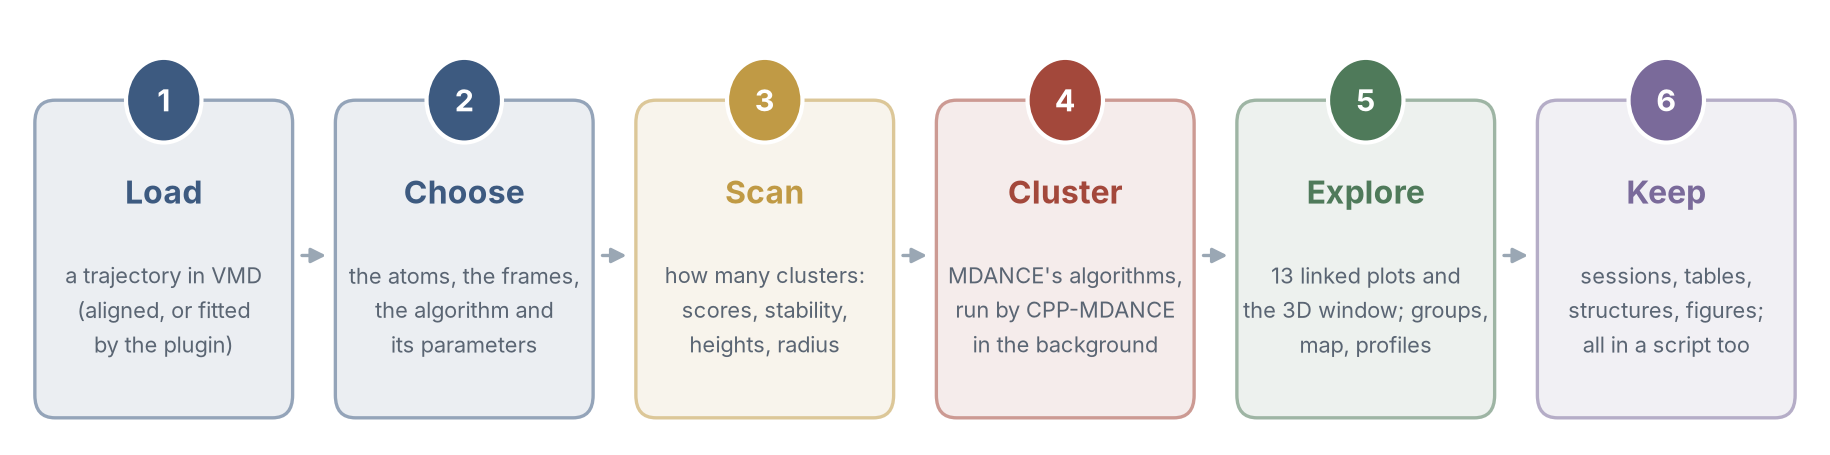
\includegraphics[width=\textwidth]{workflow.png}
  \caption{A clustering with VMDance, from the trajectory to what is kept.}
  \label{fig:workflow}
\end{figure}

% ---------------------------------------------------------------------------
\section{Install}
\label{sec:install}

\begin{note}
VMDance and CPP-MDANCE are to be distributed with VMD~2.x. Until then, you
install them yourself: build CPP-MDANCE, then add the plugin to VMD. The
plugin is Tcl/Tk: there is nothing to build.
\end{note}

\subsection{What you need}

\begin{center}
\small
\begin{tabularx}{\textwidth}{@{}p{0.31\textwidth}L@{}}
\toprule
\textbf{What} & \textbf{Why} \\
\midrule
VMD 2.x, built with Tcl/Tk 8.6 & The host. \cmd{info patchlevel} in VMD's
  console must say 8.6. VMD 1.9.3 has Tcl 8.5, and cannot load the plugin. \\
CMake 3.15 or later, a C++17 compiler, git & To build CPP-MDANCE. The build
  downloads Eigen 3.4 and GoogleTest when they are not installed. \\
Ghostscript (optional) & Figures in PDF and PNG. EPS works without it. \\
Tcl 8.6's headers and stub library (optional) & CPP-MDANCE's library, loaded
  into VMD. Its program alone is enough. \\
BitQT's \file{examples} folder & This guide's example: two files, cloned or
  downloaded (Section~\ref{sec:example}). \\
\bottomrule
\end{tabularx}
\end{center}

On Linux (Debian, Ubuntu), and on macOS with Homebrew, after
\cmd{xcode-select --install}:

\begin{lstlisting}[style=sh]
sudo apt install build-essential cmake git ghostscript tcl8.6-dev   # Linux
brew install cmake ghostscript tcl-tk@8                            # macOS
\end{lstlisting}

Windows takes a few more steps (a MinGW-w64 GCC, and its runtime first on the
\cmd{PATH}). The online page \emph{Install} gives them.

\subsection{Build CPP-MDANCE}

\begin{lstlisting}[style=sh]
git clone https://github.com/mqcomplab/CPP-MDANCE.git
cd CPP-MDANCE
cmake -S . -B build -DCMAKE_BUILD_TYPE=Release
cmake --build build -j
ctest --test-dir build --output-on-failure
\end{lstlisting}

This makes the program \file{build/cli/mdance-cli}, which is all VMDance needs.
It runs in the background: VMD stays usable, and \ui{Cancel} stops it.

\begin{warning}
\textbf{Eigen 5.} Homebrew's \cmd{eigen} is now version 5, which does not
compile CPP-MDANCE: the build stops at \emph{no member named `all' in
namespace `Eigen'}. Add \cmd{-DCMAKE\_DISABLE\_FIND\_PACKAGE\_Eigen3=ON} to
the first \cmd{cmake} line. The build then downloads Eigen 3.4.0 for itself.
\end{warning}

\textbf{The library} (optional). \cmd{-DBUILD\_TCL=ON} also makes
\file{build/tcl/mdance_tcl.so} (\cmd{.dylib} on macOS, \cmd{.dll} on
Windows), which VMD loads. A call then blocks VMD until it returns, and cannot
be cancelled, and it is not faster (Section~\ref{sec:bench}). Homebrew's \cmd{tcl-tk} is Tcl~9: on macOS, give CMake its Tcl
8.6.

\begin{lstlisting}[style=sh]
T=$(brew --prefix tcl-tk@8)
cmake -S . -B build -DCMAKE_BUILD_TYPE=Release -DBUILD_TCL=ON \
  -DTCL_INCLUDE_PATH=$T/include/tcl-tk -DTCL_LIBRARY=$T/lib/libtcl8.6.dylib \
  -DTCL_STUB_LIBRARY=$T/lib/libtclstub8.6.a -DTCL_TCLSH=$T/bin/tclsh8.6
\end{lstlisting}

\subsection{Add the plugin to VMD}

Get the plugin (\cmd{git clone https://github.com/diegoenry/vmd-mdance-plugin.git}),
then add three lines to your \cmd{\textasciitilde/.vmdrc}:

\begin{lstlisting}[style=tcl]
lappend auto_path /path/to/vmd-mdance-plugin/vmdance
package require vmdance   ;# adds the menu entry Analysis > VMDance
set env(MDANCE_CLI) /path/to/CPP-MDANCE/build/cli/mdance-cli
\end{lstlisting}

The last line tells the plugin where the program is. \ui{Settings}\then\ui{Backend},
in the window, chooses another build and keeps it.

\subsection{Check}

Start VMD, and type \cmd{vmdance backend} in its console. The answer names the
program, and the algorithms it was built with:

\begin{lstlisting}[style=tcl]
vmdance backend
;# mode auto ... using {cli /path/to/mdance-cli} algorithms {kmeans divine helm equal} ...
\end{lstlisting}

DIVINE is missing from a CPP-MDANCE older than its PR \#52 (October 2026).
Update it, and build it again.

% ---------------------------------------------------------------------------
\section{The example: a tau peptide, from BitQT}
\label{sec:example}

The \file{examples} folder of BitQT's repository holds a trajectory of a
flexible twelve-residue tau peptide, its ends capped: \file{aligned_tau.pdb}
and \file{aligned_original_tau_6K.dcd}, \qsFrames\ frames. Clone the
repository, or download the two files:

\begin{lstlisting}[style=sh]
git clone https://github.com/LQCT/BitQT.git      # the files: BitQT/examples
# or the two files alone:
curl -LO https://raw.githubusercontent.com/LQCT/BitQT/master/examples/aligned_tau.pdb
curl -LO https://raw.githubusercontent.com/LQCT/BitQT/master/examples/aligned_original_tau_6K.dcd
\end{lstlisting}

The same two files ship with MDANCE's Python package, whose own tutorial
clusters them too. This guide superposes the frames on one of them, frame
\qsFitFrame, before it clusters them.

% ---------------------------------------------------------------------------
\section{In the window}
\label{sec:window}

\begin{figure}[t]
  \centering
  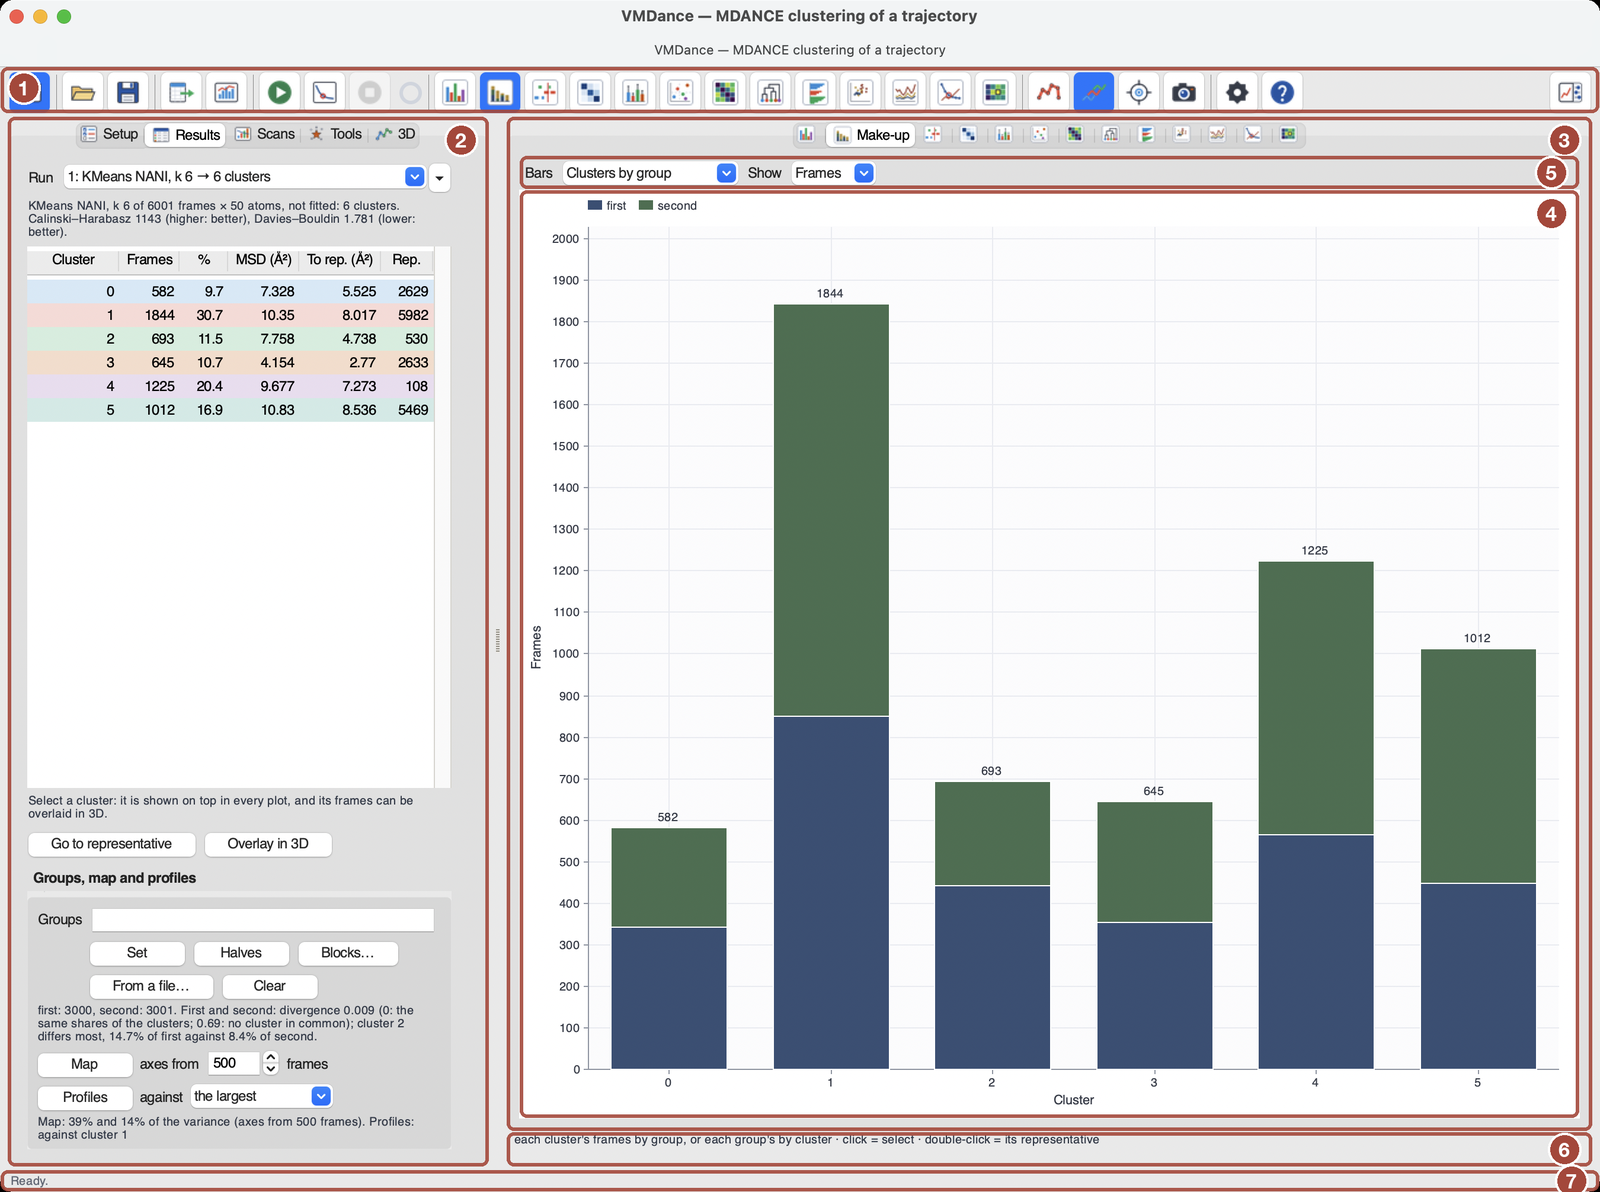
\includegraphics[width=\textwidth]{window_annotated.png}
  \caption{The VMDance window (macOS), with this guide's clustering: the
    Results pane, and the Make-up of the trajectory's two halves. (1) The
    toolbar; (2) the panes: Setup, Results, Scans, Tools, 3D; (3) the plots'
    tabs; (4) the plot; (5) its options; (6) what the pointer is on; (7) the
    status line.}
  \label{fig:window}
\end{figure}

\begin{enumerate}[leftmargin=*,label=\textbf{\arabic*.},itemsep=0.6ex]
\item \textbf{Load the trajectory.} In VMD, \ui{File}\then\ui{New Molecule}:
  load \file{aligned_tau.pdb}, then \file{aligned_original_tau_6K.dcd} into
  the same molecule. The PDB is the topology: it names the atoms. Its
  coordinates come in as frame 0, which is not part of the trajectory. Delete
  that first frame: type \cmd{animate delete beg 0 end 0} in VMD's console.
  The molecule then has the DCD's \qsFrames\ frames.
\item \textbf{Fit the frames to frame \qsFitFrame}, on the atoms to cluster.
  Setup's \ui{Fit to the first frame} superposes the frames on the first one
  clustered; to fit them on another, do it in VMD's console first (the lines
  of Listing~\ref{lst:script}, step 3):
\begin{lstlisting}[style=tcl]
set sel "resid 3 to 12 and name N CA C O H"
set ref [atomselect top $sel frame 999]
set fit [atomselect top $sel]
set all [atomselect top all]
for {set f 0} {$f < [molinfo top get numframes]} {incr f} {
    $fit frame $f; $all frame $f; $all move [measure fit $fit $ref]
}
\end{lstlisting}
  VMD's coordinates move: every frame, whole molecule, is superposed on frame
  \qsFitFrame\ by those atoms. VMD may print \emph{Matrix: Warning: no
  convergence} for some of them. Its fit is then still within
  \qsFitWorst\,\AA\ of the best one here.
\item \textbf{Open VMDance}: \ui{Analysis}\then\ui{VMDance} (in VMD 1.9,
  \ui{Extensions}\then\ui{Analysis}\then\ui{VMDance}), or type \cmd{vmdance}
  in VMD's console. Figure~\ref{fig:window} names its parts.
\item \textbf{Choose what to cluster}, in \ui{Setup}\then\ui{What to cluster}.
  Atoms: \cmd{resid 3 to 12 and name N CA C O H}, the backbone of residues 3
  to 12 and its amide hydrogens (\qsAtoms\ atoms). The atoms decide what
  ``alike'' means: here, the peptide's fold.

  Leave \ui{Fit to the first frame} off: the frames are fitted already. The
  note under it compares a sample of them with the first: \qsAsIs\,\AA\ as they
  are, \qsFitted\,\AA\ once fitted. They look superposed. (Frames that are not
  would come far nearer once fitted: the note would turn red-brown.) The run's
  summary will say \emph{not fitted}: the plugin's own fit is off.
\item \textbf{Choose the algorithm}, in \ui{Setup}\then\ui{Algorithm}: KMeans
  NANI, with \ui{Seeding} set to \ui{Complementary similarity}
  (\cmd{CompSim}). NANI then draws its seeds from the densest frames.
\item \textbf{Ask how many clusters}, in \ui{Scans}\then\ui{Elbow}: k from 2 to
  12, tick \ui{Stability}, and press \ui{Scan}. The scan clusters at every k.
  It does so again from NANI's four seedings that draw no random number, to
  see whether the clusters depend on the seeding.
\item \textbf{Read the scan} (the Elbow plot, Figure~\ref{fig:gallery}M). It
  rings the values the scores point to, and the Scans box says them in words.
  Section~\ref{sec:reading} reads them. Double-click k~\qsK\ in the plot: it
  becomes the clustering, a run of its own.
\item \textbf{Read the clusters.} \ui{Results} holds their table: frames,
  share, MSD, representative frame. Click a cluster: it is drawn on top in
  every plot. Double-click it: VMD goes to its representative frame. The plots
  are on the right (Section~\ref{sec:gallery}). Hover one: the line under it
  says what the pointer is on.
\item \textbf{See them in 3D.} \ui{3D}\then\ui{Colour by cluster}, then play the
  trajectory: the structure takes the colour of the current frame's cluster.
  \ui{Representatives} draws them all at once (Figure~\ref{fig:reps}).
\item \textbf{Compare the two halves of the run}, in
  \ui{Results}\then\ui{Groups, map and profiles}: press \ui{Halves}. The
  \ui{Make-up} plot shows each cluster by half (Figure~\ref{fig:window}), and
  the line under the box says how unlike the halves are. \ui{Map} and
  \ui{Profiles}, below it, make those two plots.
\item \textbf{Keep it.} \ui{File}\then\ui{Save session} keeps every run, the
  scans and the groups. \ui{File}\then\ui{Export results} writes the tables.
  \ui{File}\then\ui{Create figures} writes the plots as PDF, PNG or EPS, sized
  for a paper's column or a slide.
\end{enumerate}

% ---------------------------------------------------------------------------
\section{In a script}
\label{sec:script}

Every step above is a VMD or \cmd{vmdance} command. The script below,
\cmd{quickstart.tcl} (beside this guide's source), runs them all. It also
asks DIVINE, HELM and eQual for a second opinion, and sweeps three algorithms
and two seedings. Run it in the folder of the two files:

\begin{lstlisting}[style=sh]
vmd -dispdev text -e quickstart.tcl
\end{lstlisting}

Or paste it, a line at a time, into VMD's console: the window, when it is
open, shows what the command did. It took about \qsMinutes\ minute(s) here
(\qsMachine), most of it the elbow scan and the sweep.

\lstinputlisting[style=tcl,caption={\cmd{quickstart.tcl}: the whole analysis of
  this guide.},label=lst:script,captionpos=b,numbers=left,numberstyle=\tiny\color{muted},
  numbersep=8pt,xleftmargin=18pt,framexleftmargin=18pt]{quickstart.tcl}

Text-mode VMD prints what each command returns, as its console does. The
\cmd{puts} lines print the rest, and the scan says how far it is as it runs.
The script leaves two things in the folder:

\begin{itemize}
  \item \file{tau_results}, the tables of the k~\qsK\ clustering. Each has a
    header saying how it was made.\\
    {\raggedright\small\ttfamily\qsExportFiles\par}
  \item \cmd{tau.vmdance}, the session (\qsSessionKB\ KB): its \qsRuns\ runs,
    the scans, the groups, the map and the profiles. \cmd{vmdance session load
    tau.vmdance} opens it again, with the window or without.
\end{itemize}

% ---------------------------------------------------------------------------
\section{What the example says}
\label{sec:reading}

\begin{table}[H]
\centering
\small
\caption{The elbow scan (Listing~\ref{lst:script}, step 4; Figure~\ref{fig:gallery}M). The stability is
  the mean adjusted Rand index of every two of NANI's four deterministic
  seedings (1: the same clusters, whatever the seeding).}
\label{tab:elbow}
\begin{tabular}{@{}rrrrr@{}}
\toprule
k & Calinski--Harabasz & Davies--Bouldin & Variance & Stability \\
  & (higher: better) & (lower: better) & explained & \\
\midrule
\qsElbowRows \\
\bottomrule
\end{tabular}
\end{table}

\textbf{How many clusters?} The Scans box says: \emph{``\qsSuggestWords''}.
These are three readings, and they do not agree.

\begin{itemize}
  \item The scores are best at k~\qsDbLowest: Davies--Bouldin is lowest there
    (\qsDbLowestValue), and Calinski--Harabasz highest (\qsChHighestValue).
    Calinski--Harabasz falls at every k, from \qsChFirst\ at k~\qsKFirst\ to
    \qsChLast\ at k~\qsKLast, as it does on structures that form no
    well-separated states. Two clusters are the best-separated partition, and
    the coarsest.
  \item Davies--Bouldin dips most sharply at k~\qsDbDip: \qsDbDipValue, between
    \qsDbDipBefore\ at k~\qsDbDipBeforeK\ and \qsDbDipAfter\ at
    k~\qsDbDipAfterK. The score bends there. The lowest value and the sharpest
    dip are MDANCE's two criteria.
  \item The seedings agree at k~\qsStable\ (stability \qsStableValues).
    From k~\qsAboveFrom\ on, the stability is between \qsAboveMin\ and
    \qsAboveMax: there another seeding gives, in part, other clusters.
\end{itemize}

None of these is wrong: they answer different questions. This guide takes
k~\qsK, as MDANCE's own tutorial does, for a finer look at the shapes the
peptide takes than two clusters give. It is where Davies--Bouldin dips most
sharply (\qsKDb; Calinski--Harabasz \qsKCh). But its stability is
\qsKStability: the four seedings do not make quite the same six clusters,
where at k~\qsStableLast\ they nearly do (\qsStableLastValue). Say so when
you report them.

\textbf{The clusters.} At k~\qsK, the clusters hold \qsSizes\ frames
(\qsPcts\%; Figure~\ref{fig:gallery}A). Their mean silhouette is
\qsSilCentroid\ from the clusters' mean structures, and \qsSilPairs\ from
every frame (Figure~\ref{fig:gallery}G). By the second, \qsSilNegative\
frames (\qsSilNegativePct\%) are nearer another cluster's frames than their
own's: the clusters are loose. The trajectory stays \qsStayMin\ to
\qsStayMax\ frames in a cluster on average before it moves on
(Figure~\ref{fig:gallery}D): the frames are far apart in time, and the
peptide changes between any two.

\textbf{Has the run converged?} Both halves of the trajectory visit all
\qsK\ clusters, but not equally (Figure~\ref{fig:gallery}B):
cluster~\qsDiffCluster\ holds \qsDiffFirstPct\% of the first half and
\qsDiffSecondPct\% of the second. The divergence of their shares is
\qsDivergence\ (0: the same shares; 0.69: no cluster in common). The halves
are alike, not the same: a longer run, or more replicas, would change the
populations.

\textbf{A second opinion.} At k~\qsK, DIVINE, which splits the frames from the
top, and HELM, which merges 60 small NANI clusters two by two, agree with
KMeans NANI in part only (adjusted Rand index \qsDivineAri\ and \qsHelmAri;
1: the same clusters). The sweep's best configuration, by Davies--Bouldin, is
\qsSweepBest\ (\qsSweepBestDb; Figure~\ref{fig:gallery}L). eQual finds as
many clusters as its radius makes: at 8\,\Asq\ (an RMSD of 4\,\AA\ to the
seed), \qsEqualClusters\ clusters. The three largest hold
\qsEqualTopThreePct\% of the frames (\qsEqualTopThree).

So the peptide's conformations form a continuum, not six states with
barriers between them. The k~\qsK\ clusters are a partition of it, useful to
look at the shapes it takes, and another seeding or algorithm draws their
borders a little otherwise. Report them with their stability and silhouette,
and set beside them k~\qsDbLowest, the best scores, and k~\qsStableLast, the
finest partition the seedings agree on.

\begin{figure}[H]
  \centering
  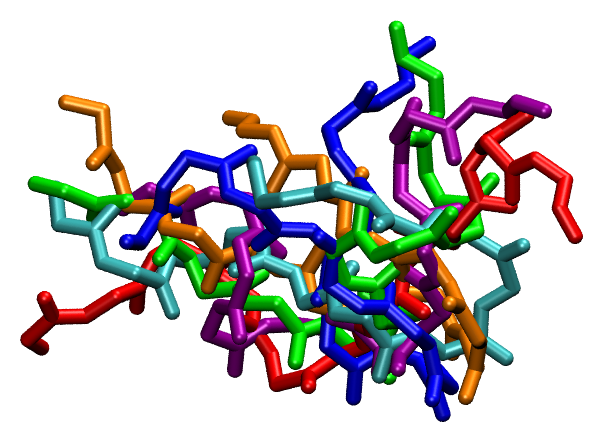
\includegraphics[width=0.58\textwidth]{main_3d.png}
  \caption{The \qsK\ clusters' representatives (frames \qsReps), each in its
    cluster's colour: \ui{3D}\then\ui{Representatives}, or \cmd{vmdance draw
    -reps 1}.}
  \label{fig:reps}
\end{figure}

% ---------------------------------------------------------------------------
\section{The 13 plots}
\label{sec:gallery}

Every plot draws the current clustering, its selected clusters on top, and
answers a question of its own. Figure~\ref{fig:gallery} shows all 13, as
\cmd{vmdance figures} writes them, for this guide's clustering. The Make-up
shows the trajectory's two halves (\cmd{vmdance groups -blocks 2}); the Map
and the Profiles show the clusters.

Hover a plot in the window: the line under it says what the pointer is on.
\ui{Plot options}\then\ui{All plots} gives the distances squared (\Asq, as
they are measured) or as lengths (\AA), and the time per frame, so that the
Timeline and the Residence read in nanoseconds.

% a panel of the gallery, its letter at its top left (#1: its width, #2: the
% plot, #3: the letter); the panels' descriptions are in the figure's caption
\newcommand{\gpanel}[3]{%
  \begin{tikzpicture}[baseline=(img.north)]
    \node[inner sep=0pt, anchor=north west] (img) at (0,0)
      {\includegraphics[width=#1]{gallery_#2.pdf}};
    \node[anchor=north west, inner sep=0pt, font=\sffamily\bfseries]
      at ([xshift=1pt, yshift=-1pt]img.north west) {#3};
  \end{tikzpicture}}
\newcommand{\half}{0.49\textwidth}

\begin{figure}[p]
  \centering
  \gpanel{\half}{populations}{A}\hfill\gpanel{\half}{makeup}{B}\\[1.2ex]
  \gpanel{\half}{transitions}{C}\hfill\gpanel{\half}{residence}{D}\\[1.2ex]
  \gpanel{\half}{compactness}{E}\hfill\gpanel{\half}{distances}{F}
  \caption{The 13 plots of this guide's clustering, KMeans NANI at k~\qsK\
    (Listing~\ref{lst:script}), as \cmd{vmdance figures} writes them, each
    cluster in its colour.
    (A)~\textbf{Populations}: how many frames each cluster holds.
    (B)~\textbf{Make-up}: where each cluster's frames came from; here, the
    first (blue) and the second (green) half of the trajectory.
    (C)~\textbf{Transitions}: from each cluster (rows), the share of its
    frames in each cluster one frame later.
    (D)~\textbf{Residence}: how long the trajectory stays in a cluster once it
    enters it (the mean, in frames).
    (E)~\textbf{Compactness}: how tight each cluster is (MDANCE's MSD within,
    \Asq).
    (F)~\textbf{Distances}: how far apart the clusters' mean structures are
    (RMSD\textsuperscript{2}, \Asq). Continued overleaf.}
  \label{fig:gallery}
\end{figure}

\begin{figure}[p]
  \ContinuedFloat
  \centering
  \gpanel{\half}{silhouette}{G}\hfill\gpanel{\half}{map}{H}\\[1.2ex]
  \gpanel{\half}{profiles}{I}\hfill\gpanel{\half}{tree}{J}\\[1.2ex]
  \gpanel{\textwidth}{timeline}{K}
  \caption{The 13 plots (continued).
    (G)~\textbf{Silhouette}: whether each frame is nearer its own cluster than
    the next, from the clusters' mean structures; dashed, the mean.
    (H)~\textbf{Map}: the frames on their first two principal components, by
    cluster; the representatives ringed.
    (I)~\textbf{Profiles}: each cluster's RMSF, residue by residue: where its
    frames move.
    (J)~\textbf{Tree}: how the clusters join: the average linkage of their
    mean structures (for HELM, its own merges).
    (K)~\textbf{Timeline}: the cluster of every frame. With more frames than
    pixels, the darker, the larger the share of the frames there that are in
    the cluster. Continued overleaf.}
\end{figure}

\begin{figure}[p]
  \ContinuedFloat
  \centering
  \gpanel{\textwidth}{sweep}{L}\\[2ex]
  \gpanel{\textwidth}{elbow}{M}
  \caption{The 13 plots (continued).
    (L)~\textbf{Sweep}: which algorithm, seeding and k score best:
    Calinski--Harabasz of three algorithms and two seedings at k 2 to 8
    (darker: higher; outlined: the best).
    (M)~\textbf{Elbow}: how many clusters. The scan of
    Listing~\ref{lst:script}, step 4: Calinski--Harabasz (blue),
    Davies--Bouldin (red) and the stability across NANI's seedings (bars);
    ringed where they point; dotted, the clustering (Table~\ref{tab:elbow}).}
\end{figure}

% ---------------------------------------------------------------------------
\section{Choosing an algorithm}
\label{sec:algorithms}

\begin{figure}[H]
  \centering
  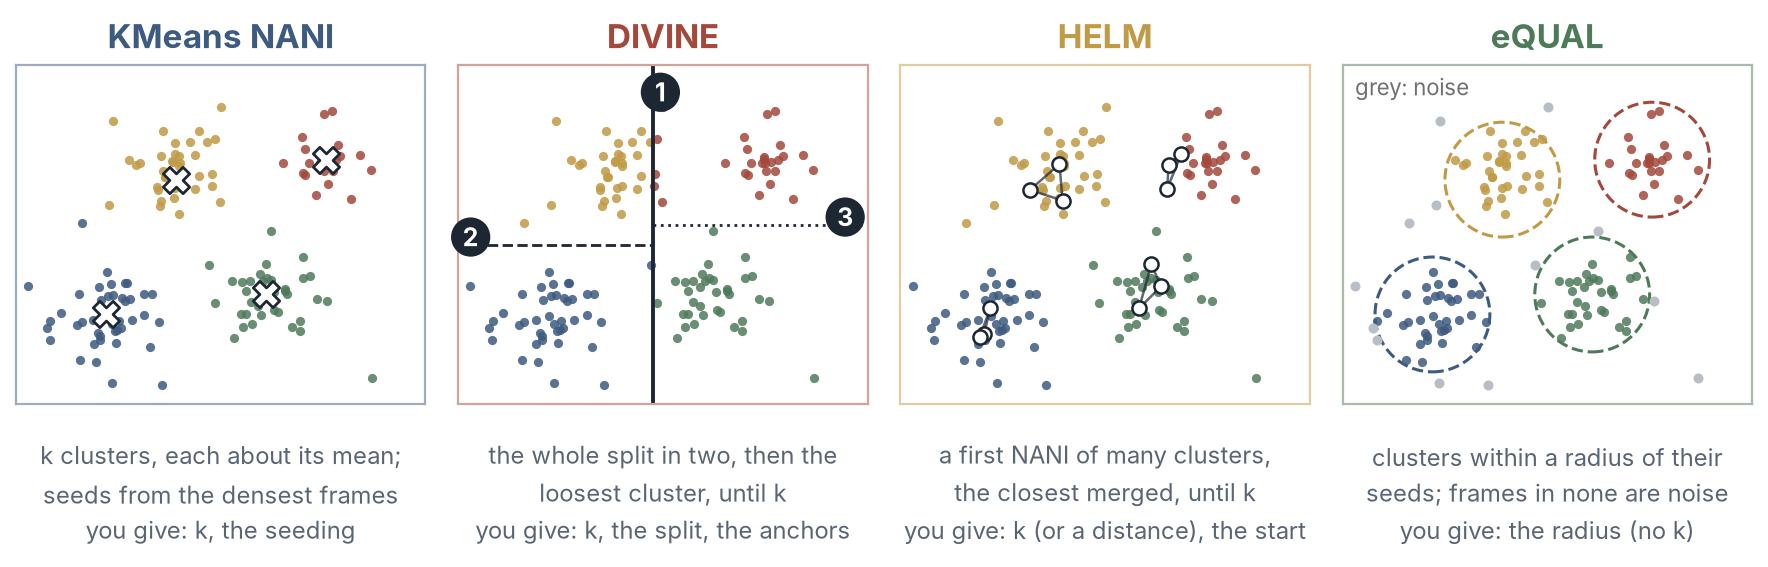
\includegraphics[width=\textwidth]{algorithms.png}
  \caption{The four algorithms on the same frames.}
  \label{fig:algorithms}
\end{figure}

\begin{table}[H]
\centering
\small
\caption{The algorithms, and their main options with their defaults. A
  parameter has \cmd{mdance-cli}'s name; \cmd{vmdance parameters \meta{algorithm}} lists them all, with their limits.}
\label{tab:algorithms}
\begin{tabularx}{\textwidth}{@{}p{0.14\textwidth}LLp{0.22\textwidth}@{}}
\toprule
\textbf{Algorithm} & \textbf{What it does} & \textbf{You give} & \textbf{Good for} \\
\midrule
KMeans NANI & k-means, its seeds drawn from the densest frames (or
  k-means++, random) & \cmd{-k 6}; \cmd{-kinit StratAll} (\cmd{StratReduced},
  \cmd{CompSim}, \cmd{DivSelect}, \cmd{KmeansPP}, \cmd{Random});
  \cmd{-percentage 10} & a first look; most trajectories; the stability scan \\
\addlinespace
DIVINE & splits the frames in two, then the loosest cluster, until k &
  \cmd{-k 6}; \cmd{-split WeightedMSD} (\cmd{MSD}, \cmd{Radius});
  \cmd{-anchors NANI} (\cmd{OutlierPair}, \cmd{SplinterPair});
  \cmd{-threshold 0}, the smallest share & a hierarchy from the top; clusters
  of very different sizes \\
\addlinespace
HELM & many small NANI clusters, merged two by two until k (or a distance) &
  \cmd{-k 6} (or \cmd{-eps}); \cmd{-initial 50} (or \cmd{-initial-labels});
  \cmd{-merge-scheme Intra} (\cmd{Inter}, \cmd{Half}); \cmd{-trim-start 0} & a
  hierarchy from the bottom; the merges' heights \\
\addlinespace
eQual & clusters within a radius of their seeds; the rest is noise &
  \cmd{-threshold 2}, the radius (MDANCE's MSD, \Asq); no k & dense states
  among sparse frames; a k it finds itself \\
\bottomrule
\end{tabularx}
\end{table}

\begin{itemize}
  \item \textbf{The frames must be superposed.} MDANCE clusters coordinates as
    they are. Frames that drift separate by where the molecule is, not by its
    shape. \cmd{-fit \meta{selection}} (\ui{Fit to the first frame}) superposes
    them on the first one clustered, and VMD's own coordinates do not move. To
    superpose them on another frame, fit them in VMD first
    (Listing~\ref{lst:script}, step 3).
  \item \textbf{The metric is MSD}, MDANCE's mean square deviation, for
    coordinates. The other indices are for fingerprint-like data; DIVINE and
    eQual take MSD only.
  \item \textbf{eQual's radius is an MSD}: half the RMSD\textsuperscript{2} of a
    frame and its seed. A frame joins when its RMSD to the seed is at most
    $\sqrt{2 \times \text{radius}}$. \cmd{vmdance radii} proposes a range from
    the frames.
  \item \textbf{An elbow scan} (\cmd{vmdance elbow}) works for every algorithm:
    by k, or by radius for eQual. A sweep (\cmd{vmdance sweep}) compares
    algorithms, seedings and k at once.
\end{itemize}

% ---------------------------------------------------------------------------
\section{The program or the library}
\label{sec:bench}

CPP-MDANCE runs as a program, \cmd{mdance-cli}, or as a library loaded into
VMD, \cmd{mdance\_tcl} (Section~\ref{sec:install}). VMDance gives both the
same coordinates, and both give the same clusters. They differ in how they
run:

\begin{itemize}
  \item The program runs in the background: VMD stays usable, and \ui{Cancel}
    stops it. The coordinates go to it as a CSV file, and its answer comes
    back as JSON.
  \item The library runs inside VMD: VMD waits until it returns, and it cannot
    be cancelled. The coordinates go to it as one Tcl list, and the CSV file
    is written all the same.
\end{itemize}

Table~\ref{tab:bench} times the two on this guide's trajectory (\bnFrames\
frames, fitted on frame \bnFitFrame), on its \bnAtomsBackbone\ backbone atoms
and on all \bnAtomsAll\ of its atoms. Each job is timed whole, as you wait
for it: the coordinates written, CPP-MDANCE, its answer read, and the
plugin's own measures of the clusters. The time is the median of \bnReps\
runs, after one not counted.

\begin{table}[H]
\centering
\small
\caption{The program against the library: seconds a job (\bnMachine, VMD
  \qsVMD, CPP-MDANCE \qsBackendCommit; \cmd{make bench} in the guide's
  folder). The last column is the program's time over the library's: below
  1, the program is the faster.}
\label{tab:bench}
\begin{tabular}{@{}lrrrr@{}}
\toprule
Job & Atoms & Program (s) & Library (s) & Program / library \\
\midrule
\bnRows \\
\bottomrule
\end{tabular}
\end{table}

\textbf{The same clusters.} All \bnCompared\ jobs gave the same answers in
both modes: the same labels and, for the scans, the same sizes and scores.

\textbf{The library is not faster.} A single clustering took longer with it:
\bnKmeansLib\ s against \bnKmeansCli\ s for KMeans NANI on the backbone,
\bnKmeansAllLib\ s against \bnKmeansAllCli\ s on every atom. The library is
given the coordinates as one Tcl list, which CPP-MDANCE's Tcl binding turns
into text, and the CSV file is written all the same. The program reads that
file instead, and starts in a moment. Only the scans, which call CPP-MDANCE
again and again with the same list, gain a little from the library: the scan
with stability, 55 clusterings, took \bnStabilityLib\ s against
\bnStabilityCli\ s. Over all the jobs, the program took \bnGainMin\ to
\bnGainMax\ times the library's time.

\textbf{The library costs memory.} Over its runs, VMD grew by \bnMemLib\ MB,
against \bnMemCli\ MB over the program's: Tcl keeps the text of the
coordinates' list, about 120 bytes a coordinate, until VMD quits.

So use the program: it is as fast, it leaves VMD usable and the job stoppable,
and VMD's memory hardly grows with it. The library is an option where no program
can be run beside VMD.

% ---------------------------------------------------------------------------
\section{The command at a glance}
\label{sec:command}

A cluster is its number (0, 1,~\ldots); a frame is VMD's frame number.
\cmd{vmdance help} lists every subcommand, and \cmd{vmdance help \meta{subcommand}} gives one's usage. Every option is checked before anything
changes, and an error names the option and what to change.

\begin{center}
\small
\begin{tabularx}{\textwidth}{@{}T{0.52\textwidth}L@{}}
\toprule
\normalfont\textbf{Command} & \textbf{What it does} \\
\midrule
vmdance & opens the window \\
vmdance -mol top -sel "name CA" -algorithm kmeans -k 6 & clusters (a new run); also \cmd{-fit}, \cmd{-first}, \cmd{-last}, \cmd{-step} and the algorithm's parameters \\
vmdance alignment | radii & do the frames look superposed? A range for eQual's radius \\
vmdance elbow -from 2 -to 12 -stability 1 & the scores (and the stability) at every k \\
vmdance elbow suggest | elbow load 3 & where the scores point; that k made the clustering \\
vmdance sweep -algorithms \{kmeans helm\} -from 2 -to 10 & every configuration; \cmd{sweep best db} \\
vmdance clusters | get 2 | labels & the table; one cluster; every frame's cluster \\
vmdance timeline | transitions -lag 10 | residence & when, where to next, how long \\
vmdance silhouette -kind pairs | distances | tree & how well separated, how far apart, how they join \\
vmdance groups -blocks 2 | groups -ranges \{a 0-99 b 100-199\} & where each frame came from \\
vmdance makeup | groups compare & each cluster by group; how unlike the groups are \\
vmdance map | profiles & the frames' principal components; RMSF by residue \\
vmdance prime | similarity & PRIME's native-like frame; each cluster's iSIM \\
vmdance pick -method diversity -param 10 & frames picked without clustering \\
vmdance select 0 | draw -colour 1 -reps 1 | goto 0 & VMD's 3D window \\
vmdance runs | run 1 | renumber & the runs kept; clusters numbered by size \\
vmdance export dir | session save file & the tables; the session \\
vmdance figures dir -plots \{populations elbow\} -size column & figures (VMD's window needed) \\
vmdance backend | help & which CPP-MDANCE is used; the subcommands \\
\bottomrule
\end{tabularx}
\end{center}

% ---------------------------------------------------------------------------
\section{What to report}
\label{sec:report}

Whoever reads your clustering needs:

\begin{itemize}
  \item the atoms, and the superposition: fitted or not, on which atoms, and
    onto which frame (here frame \qsFitFrame, in VMD, before clustering: the
    plugin's own fit was off);
  \item the frames (all, a range, every n-th) and their time apart;
  \item the algorithm, its parameters, and the backend: CPP-MDANCE's version or
    commit;
  \item how k was chosen: which reading of the scores, the stability, a second
    algorithm's view;
  \item the clusters' sizes and silhouette, and which silhouette;
  \item with groups, each cluster's make-up.
\end{itemize}

The exported tables carry most of it in their headers (\file{tau_summary.txt}
here). Cite the algorithms you used, MDANCE, CPP-MDANCE and VMD
(\hyperref[sec:references]{References}, page~\pageref{sec:references}).

% ---------------------------------------------------------------------------
\section{When something goes wrong}
\label{sec:problems}

\begin{center}
\small
\begin{tabularx}{\textwidth}{@{}p{0.36\textwidth}L@{}}
\toprule
\textbf{What you see} & \textbf{What to do} \\
\midrule
CPP-MDANCE's build stops at \emph{no member named `all' in namespace `Eigen'}
  & Eigen 5 is installed: add \cmd{-DCMAKE\_DISABLE\_FIND\_PACKAGE\_Eigen3=ON}
  (Section~\ref{sec:install}). \\
\addlinespace
\emph{no MDANCE backend was found} & Build CPP-MDANCE, and set
  \cmd{MDANCE\_CLI} in \cmd{\textasciitilde/.vmdrc}, or choose it in
  \ui{Settings}\then\ui{Backend}. \\
\addlinespace
VMD cannot load the plugin: it needs Tcl 8.6 & VMD 1.9.3 has Tcl 8.5: use VMD 2. \\
\addlinespace
VMD has no Extensions menu & VMD 2's main window has none: \ui{Analysis}\then\ui{VMDance}. \\
\addlinespace
DIVINE is not offered & CPP-MDANCE is older than its PR \#52: update it, and build it again. \\
\addlinespace
The molecule has 6002 frames, not 6001 & The PDB's own frame:
  \cmd{animate delete beg 0 end 0}. \\
\addlinespace
The note under \ui{Fit to the first frame} turns red-brown & The frames are not
  superposed: tick the box (\cmd{-fit \meta{selection}}). \\
\addlinespace
\emph{-k 10: NANI \ldots\ seeds its 10 clusters from the densest 10\% of the 60 frames}
  & Raise \ui{Seeds from \%} (\cmd{-percentage}), cluster more frames, ask for
  fewer clusters, or seed with \cmd{KmeansPP}. \\
\addlinespace
\cmd{figures} fails in text-mode VMD & Figures are drawn by Tk: run VMD with
  its window (\cmd{vmd -e script.tcl}). PDF and PNG also need Ghostscript. \\
\bottomrule
\end{tabularx}
\end{center}

Every message names the option to change, and the window adds the field it
is. The online page \emph{Questions} answers more.

% ---------------------------------------------------------------------------
\section{Further reading}

The online documentation, \url{https://diegoenry.github.io/vmd-mdance-plugin/},
goes further: a complete analysis of the tau peptide (HELM's merges' heights,
eQual's radii, the map and the profiles), the window pane by pane, every
parameter, every plot, the command, the files, and the plugin's limits.

\section*{References}
\phantomsection\label{sec:references}
\addcontentsline{toc}{section}{References}

{\small
\begin{enumerate}[label={[\arabic*]},leftmargin=*,itemsep=0.3ex]
\item \textbf{MDANCE.} Chen, L.; Miranda-Quintana, R. A. MDANCE: Flexible and
  Versatile N-ary Clustering Package. \emph{Biophys. J.} \textbf{2025}, 124,
  485a. \url{https://doi.org/10.1016/j.bpj.2024.11.2557};
  \url{https://github.com/mqcomplab/MDANCE}
\item \textbf{CPP-MDANCE}, the C++ implementation of MDANCE that runs the
  clustering. \url{https://github.com/mqcomplab/CPP-MDANCE}
\item \textbf{KMeans NANI.} Chen, L.; Roe, D. R.; Kochert, M.; Simmerling, C.;
  Miranda-Quintana, R. A. k-Means NANI: An Improved Clustering Algorithm for
  Molecular Dynamics Simulations. \emph{J. Chem. Theory Comput.}
  \textbf{2024}, 20, 5583--5597. \url{https://doi.org/10.1021/acs.jctc.4c00308}
\item \textbf{DIVINE.} Santos, J. B. W.; Chen, L.; Miranda-Quintana, R. A.
  Divide and Cluster: The DIVINE Framework for Deterministic Top-Down Analysis
  of Molecular Dynamics Trajectories. \emph{bioRxiv} \textbf{2025}.
  \url{https://doi.org/10.1101/2025.06.20.660828}
\item \textbf{HELM.} Chen, L.; Santos, J. B. W.; Gaza, J.; Perez, A.;
  Miranda-Quintana, R. A. Hierarchical Extended Linkage Method (HELM)'s Deep
  Dive into Hybrid Clustering Strategies. \emph{J. Chem. Inf. Model.}
  \textbf{2025}, 65, 6209--6220. \url{https://doi.org/10.1021/acs.jcim.5c00539}
\item \textbf{eQual.} Chen, L.; Smith, M.; Roe, D. R.; Miranda-Quintana, R. A.
  Extended Quality (eQual): Radial Threshold Clustering Based on n-ary
  Similarity. \emph{J. Chem. Inf. Model.} \textbf{2025}, 65, 5062--5070.
  \url{https://doi.org/10.1021/acs.jcim.4c02341}
\item \textbf{BitQT}, whose examples hold this guide's trajectory.
  Gonz\'alez-Alem\'an, R.; Platero-Rochart, D.; Hern\'andez-Castillo, D.;
  Hern\'andez-Rodr\'iguez, E. W.; Caballero, J.; Leclerc, F.;
  Montero-Cabrera, L. BitQT: A Graph-Based Approach to the Quality Threshold
  Clustering of Molecular Dynamics. \emph{Bioinformatics} \textbf{2022}, 38,
  73--79. \url{https://doi.org/10.1093/bioinformatics/btab595};
  \url{https://github.com/LQCT/BitQT}
\item \textbf{VMD.} Humphrey, W.; Dalke, A.; Schulten, K. VMD: Visual
  Molecular Dynamics. \emph{J. Mol. Graphics} \textbf{1996}, 14, 33--38.
  \url{https://doi.org/10.1016/0263-7855(96)00018-5}
\item \textbf{Calinski--Harabasz.} Cali\'nski, T.; Harabasz, J. A Dendrite
  Method for Cluster Analysis. \emph{Commun. Stat.} \textbf{1974}, 3, 1--27.
  \url{https://doi.org/10.1080/03610927408827101}
\item \textbf{Davies--Bouldin.} Davies, D. L.; Bouldin, D. W. A Cluster
  Separation Measure. \emph{IEEE Trans. Pattern Anal. Mach. Intell.}
  \textbf{1979}, PAMI-1, 224--227. \url{https://doi.org/10.1109/TPAMI.1979.4766909}
\item \textbf{The silhouette.} Rousseeuw, P. J. Silhouettes: A Graphical Aid to
  the Interpretation and Validation of Cluster Analysis. \emph{J. Comput.
  Appl. Math.} \textbf{1987}, 20, 53--65.
  \url{https://doi.org/10.1016/0377-0427(87)90125-7}
\item \textbf{The adjusted Rand index}, for the stability. Hubert, L.; Arabie,
  P. Comparing Partitions. \emph{J. Classif.} \textbf{1985}, 2, 193--218.
  \url{https://doi.org/10.1007/BF01908075}
\end{enumerate}
}

\vfill
{\footnotesize\color{muted}
Every number in this guide was made by its own script
(Listing~\ref{lst:script}), with VMDance \qsVersion, CPP-MDANCE (commit
\qsBackendCommit) and VMD \qsVMD\ on \qsArch\ (\qsMachine). The guide's
source is in the plugin's repository, in \cmd{quickstart-guide/}: \cmd{make
check} there makes its numbers again, and compares them with these.\par}

\end{document}
